% Neuroloop utilities - Library reference - Top level
% Written by Christopher Thomas.

\documentclass[letterpaper,11pt]{report}
\usepackage[letterpaper]{geometry}
\usepackage{graphicx}
\usepackage{verbatim}
\usepackage{placeins}
\usepackage{longtable}

\geometry{nohead,footskip=0.3in,margin=0.75in}

% Force my paragraph style, darnit.
\usepackage{indentfirst}
\setlength{\parskip}{\baselineskip}

% NOTE - "\thispagestyle" is used for part and chapter beginning pages, and
% overrides \pagestyle. Redefine it to be harmless.
% NOTE - The canonical solution ("\pagenumbering{gobble}") resets the page
% counter whenever it's used.
\renewcommand{\thispagestyle}[1]{}

% Custom macros.
\newcommand{\fixme}[1]{\textbf{FIXME: #1}}

\newcommand{\figdef}[3]
{\begin{figure}[htb]
\begin{center}#1\end{center}
\caption{#2}\label{#3}\end{figure}}

\newcommand{\tabdef}[3]
{\begin{table}[hb]
\begin{center}#1\end{center}
\caption{#2}\label{#3}\end{table}}

% Document body.
\begin{document}
%
% Title page.
%
\pagestyle{empty}

\begin{center}
%
\vspace*{1in}
{\Huge NeuroLoop Utilities -- Function Reference} \\
{\footnotesize Written by Christopher Thomas -- \today.}
%
\vspace*{1in}\\
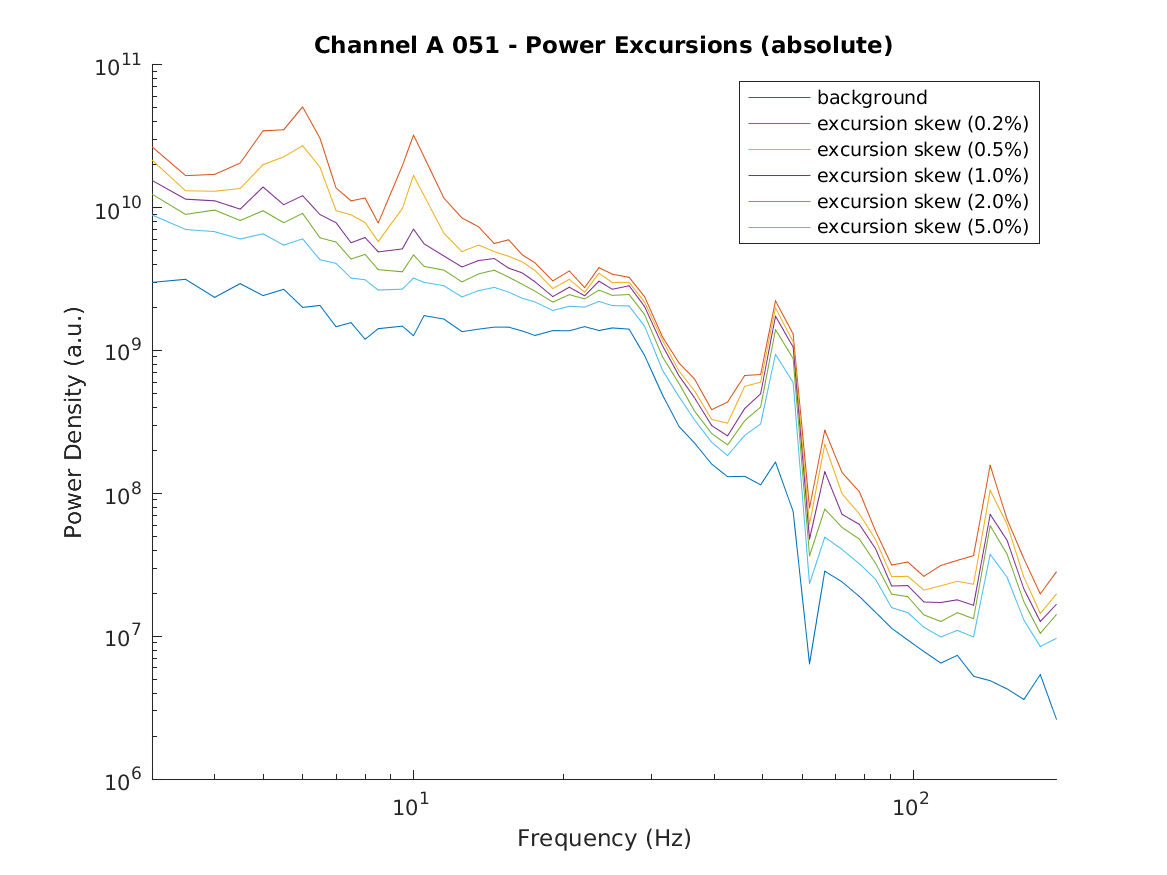
\includegraphics[width=6in]{plots/20201005/spect-burst-abs-A-051}
%
\end{center}
%
\vfill
{\tiny \input{../LICENSE.md}}
%
\clearpage
%
%
% Front matter.
%
\pagestyle{plain}
\pagenumbering{roman}
\setcounter{page}{1}
%
\tableofcontents
%
\clearpage
%
%
% Document parts.
%
\pagestyle{plain}
\setcounter{page}{1}
\pagenumbering{arabic}
%
% Neuroloop utilities - Library reference - Overview
% Written by Christopher Thomas.

\chapter{Overview}
\label{sect-over}

The NeuroLoop utility library functions are divided into several categories:

\begin{itemize}

\item \textbf{``Processing''} functions (ch. \ref{sect-proc}) perform signal
processing operations on data series such as filtering, artifact rejection,
statistical calculations, and so forth.

\item \textbf{``Utility''} functions (ch. \ref{sect-util}) perform
miscellaneous operations that are not covered by the other categories.

\item \textbf{``Plotting''} functions (ch. \ref{sect-plot}) render plots
of various types to files, figures, or axes. These are included as an aid
to rapid prototyping, and are used by the GUI scripts. The output is
generally not publication-ready.

\item \textbf{``I/O''} functions (ch. \ref{sect-io}) facilitate operations
for reading and writing data that aren't vendor-specific.

\item \textbf{``Intan''} functions (ch. \ref{sect-intan}) facilitate the use
of datasets stored in Intan's format.

\item \textbf{``Vendor-Supplied Intan''} functions
(ch. \ref{sect-vend-intan}) are functions derived from vendor-supplied code
that are in turn wrapped by the functions in ch. \ref{sect-intan}.

\item \textbf{``Channel Tool''} functions (ch. \ref{sect-chan}) perform
operations used by the ``Channel Tool'' utility. The intention is that all
operations that are not tied to GUI implementation are packaged as library
functions for reuse outside of that application.

\end{itemize}

Several types of structure and several types of function handle are used by
the library functions. These are described in Chapter \ref{sect-notes}.

Sample code is provided in Chapter \ref{sect-examples}.

%
% This is the end of the file.

% Automatically generated documentation.
\chapter{Special Structures and Function Handles}
\label{sect-notes}

\section{CHANLIST.txt}

\verbatiminput{../lib-nloop-intan/CHANLIST.txt}

% This is the end of the file.

% Automatically generated documentation.
\chapter{``nlProc'' Functions}
\label{sect-proc}

\section{nlProc\_calcSkewPercentile.m}

\begin{verbatim}
% function [ seriesmedian seriesiqr seriesskew rawpercentiles ] = ...
%   nlProc_calcSkewPercentile(dataseries, tailpercent)
%
% This computes the median and the (tailpercent, 100%-tailpercent) tail
% percentiles for the specified series, and evaluates skew by comparing the
% midsummary (average of the tail values) with the median. The result is
% normalized (a skew of +/- 1 is a displacement by +/- the interquartile
% range).
%
% "dataseries" is the sample sequence to process.
% "tailpercent" is an array of tail values to test.
%
% "seriesmedian" is the series median value.
% "seriesiqr" is the series interquartile range.
% "seriesskew" is an array of normalized skew values corresponding to the
%   tail percentages.
% "rawpercentiles" is an array with the actual percentile values used for
%   skew calculations. It contains percentile values corresponding to
%   [ (tailpercent) (median) (100 - tailpercent) (25%) (75%) ].
\end{verbatim}

\section{nlProc\_calcSpectrumSkew.m}

\begin{verbatim}
% function [ spectfreqs spectmedian spectiqr spectskew ] = ...
%   nlProc_calcSpectrumSkew( dataseries, samprate, ...
%   freqrange, freqperdecade, wintime, winsteps, tailpercent)
%
% This computes a persistence spectrum for the specified series, and finds
% the median, interquartile range, and the normalized skew for each frequency
% bin. "Skew" is defined per nlProc_calcSkewPercentile().
%
% "dataseries" is the data series to process.
% "samprate" is the sampling rate of the data series.
% "freqrange" [ fmin fmax ] specifies the frequency band to evaluate.
% "freqperdecade" is the number of frequency bins per decade.
% "wintime" is the window duration in seconds to compute the time-windowed
%   Fourier transform with.
% "winsteps" is the number of overlapping steps taken when advancing the time
%   window. The window advances by wintime/winsteps seconds per step.
% "tailpercent" is an array of percentile values that define the tails for
%   skew calculation, per nlProc_calcSkewPercentile().
%
% "spectfreqs" is an array of bin center frequencies.
% "spectmedian" is an array of per-frequency median power values.
% "spectiqr" is an array of per-frequency power interquartile ranges.
% "spectskew" is a cell array, with one cell per "tailpercent" value. Each
%   cell contains an array of per-frequency skew values.
\end{verbatim}

\section{nlProc\_fillNaN.m}

\begin{verbatim}
% function newseries = nlProc_fillNaN( oldseries )
%
% This interpolates NaN segments within the series using linear interpolation,
% and then fills in NaNs at the end of the series by replicating samples.
% This makes the derivative discontinuous when filling endpoints but prevents
% large excursions from curve fit extrapolation.
%
% "oldseries" is the series containing NaN segments.
%
% "newseries" is the interpolated series without NaN segments.
\end{verbatim}

\section{nlProc\_filterSignal.m}

\begin{verbatim}
% function [ lfpseries spikeseries ] = nlProc_filterSignal( oldseries, ...
%   samprate, lfprate, lowpassfreq, powerfreq, dcfreq )
%
% This applies several filters:
% - A DC removal filter.
% - A notch filter to remove power line noise.
% - A low-pass filter to isolate the local field potential signal.
% The full-rate LFP series is subtracted from the original series to produce
% a high-pass-filtered "spike" series, and a downsampled LFP series is
% also returned.
%
% "oldseries" is the original wideband signal.
% "samprate" is the sampling rate of the wideband signal.
% "lfprate" is the desired sampling rate of the LFP signal. This should
%   cleanly divide "samprate" (samprate = k * lfprate for some integer k).
% "lowpassfreq" is the edge of the pass-band for the LFP signal. This is
%   lower than the filter's corner frequency; it's the 0.2 dB frequency.
% "powerfreq" is an array of values specifying the center frequencies of the
%   power line notch filter. This is typically 60 Hz or 50 Hz (a single
%   value), but may contain multiple values to filter harmonics. An empty
%   array disables this filter.
% "dcfreq" is the edge of the pass-band for the high-pass DC removal filter.
%   Set to 0 to disable this filter. This is higher than the corner frequency;
%   it's the 0.2 dB frequency (ripple is flat above it).
%
% "lfpseries" is the downsampled low-pass-filtered signal.
% "spikeseries" is the full-rate high-pass-filtered signal.
%
% Filters used are IIR, called with "filtfilt" to remove time offset by
% running the filter forwards and backwards in time. The power line filter
% takes about 1/2 second to fully stabilize, and the low-pass LFP filter takes
% about 1/2 period to 1 period to fully stabilize. Edge effects may occur
% within this distance of the start and end of the signal.
% The DC rejection filter also takes at least 1 period to stabilize. Since
% it's applied in both directions, and won't perturb the pass-band, it should
% be well-behaved over the entire signal.
%
% The LFP sampling rate should be at least 10 times "lowpassfreq" to avoid
% aliasing during downsampling. The DC rejection filter pass frequency
% should be no lower than half the lowest frequency of interest, to
% minimize edge effects.
\end{verbatim}

\section{nlProc\_removeArtifactsSigma.m}

\begin{verbatim}
% function newseries = nlProc_removeArtifactsSigma( oldseries, ...
%   ampthresh, derivthresh, ampthreshfall, derivthreshfall, ...
%   trimbefore, trimafter, smoothsamps, dcsamps )
%
% This identifies artifacts as excursions in the signal's amplitude or
% derivative, and replaces affected regions with NaN. Excursion thresholds
% are expressed in terms of the standard deviation of the signal or its
% derivative.
%
% "oldseries" is the series to process.
% "ampthresh" is the threshold for flagging amplitude excursion artifacts.
% "derivthresh" is the threshold for flagging derivative excursion artifacts.
% "ampthreshfall" is the turn-off threshold for amplitude artifacts.
% "derivthreshfall" is the turn-off threshold for derivative artifacts.
% "trimbefore" is the number of samples to squash ahead of the artifact.
% "trimafter" is the number of samples to squash after the artifact.
% "smoothsamps" is the size of the smoothing window to apply before taking
%   the derivative, or 0 for no smoothing.
% "dcsamps" is the size of the window for computing local DC average removal
%   ahead of computing signal statistics.
%
% Regions where the amplitude or derivative exceeds the threshold are flagged
% as artifacts. These regions are widened to encompass the region where the
% amplitude or derivative exceeds the "fall" threshold, and then padded by
% the specified number of samples. This is intended to correctly handle
% square-pulse artifacts and fast-step-slow-decay artifacts.
\end{verbatim}

\section{nlProc\_removeTimeRanges.m}

\begin{verbatim}
% function newseries = ...
%   nlProc_removeTimeRanges( oldseries, samprate, trimtimes )
%
% This NaNs out specified regions of the input signal.
%
% "oldseries" is the series to process.
% "samprate" is the sampling rate of the input signal.
% "trimtimes" is a cell array containing time spans to NaN out. Time spans
%   have the form "[ time1 time2 ]", where times are in seconds. Negative
%   times are relative to the end of the signal, positive times are relative
%   to the start of the signal (both start at 0 seconds). Use a very small
%   negative value for "-0".
%
% "newseries" is a modified version of the input series with the specified
%   time ranges set to NaN.
\end{verbatim}

\section{nlProc\_trimEndpoints.m}

\begin{verbatim}
% function newseries = ...
%   nlProc_trimEndpints( oldseries, samprate, trimstart, trimend )
%
% This crops the specified durations from the start and end of the supplied
% signal.
%
% "oldseries" is the series to process.
% "samprate" is the sampling rate of the input signal.
% "trimstart" is the number of seconds to remove from the beginning.
% "trimend" is the number of seconds to remove from the end.
%
% "newseries" is a truncated version of the input signal.
\end{verbatim}

% This is the end of the file.

% Automatically generated documentation.
\chapter{``nlUtil'' Functions}
\label{sect-util}

\section{nlUtil\_readBinaryFile.m}

\begin{verbatim}
% function [is_ok sampdata] = nlUtil_readBinaryFile(fname, dtype)
%
% This attempts to read a packed array of the specified data type from the
% specified file.
%
% "fname" is the name of the file to read from.
% "dtype" is a string identifying the Matlab data type (e.g. 'uint32').
%
% "is_ok" is set to true if the operation succeeds and false otherwise.
% "sampdata" is an array containing the sample values.
\end{verbatim}

% This is the end of the file.

% Automatically generated documentation.
\chapter{``nlPlot'' Functions}
\label{sect-plot}

\section{nlPlot\_axesPlotExcursions.m}

\begin{verbatim}
% function nlPlot_axesPlotExcursions( thisax, ...
%   spectfreqs, spectmedian, spectiqr, spectskew, percentlist, ...
%   want_relative, figtitle )
%
% This plots LFP power excursions, either as relative power excess alone or
% against the median power spectrum. See nlChan_applySpectSkewCalc() for
% details of skew calculation and array contents.
% The plot is rendered to the specifed set of figure axes.
%
% "thisax" is the "axes" object to render to.
% "spectfreqs" is an array of frequency bin center frequencies.
% "spectmedian" is an array of per-frequency median power values.
% "spectiqr" is an array of per-frequency power interquartile ranges.
% "spectskew" is a cell array, with one cell per "percentlist" value. Each
%   cell contains an array of per-frequency skew values.
% "percentlist" is an array of percentile values that define the tails for
%   skew calculations, per nlProc_calcSkewPercentile().
% "want_relative" is true to plot relative power excess alone, and false to
%   plot against the median power spectrum.
% "figtitle" is the title to use for the figure, or '' for no title.
\end{verbatim}

\section{nlPlot\_axesPlotPersist.m}

\begin{verbatim}
% function nlPlot_plotPersist( thisax, ...
%   persistvals, persistfreqs, persistpowers, want_log, figtitle )
%
% This plots a pre-tabulated persistence spectrum. See "pspectrum()" for
% details of input array structure.
%
% "thisax" is the "axes" object to render to.
% "thisfig" is the figure to render to (this may be a UI component).
% "persistvals" is the matrix of persistence spectrum fraction values.
% "persistfreqs" is the list of frequencies used for binning.
% "persistpowers" is the list of power magnitudes used for binning.
% "want_log" is true if the frequency axis should be plotted on a log scale
%   (it's computed on a linear scale).
% "figtitle" is the title to use for the figure, or '' for no title.
\end{verbatim}

\section{nlPlot\_axesPlotSpikeHist.m}

\begin{verbatim}
% function nlPlot_plotSpikeHist( thisax, ...
%   bincounts, binedges, percentamps, percentpers, figtitle )
%
% This plots a pre-tabulated histogram of normalized spike waveform
% amplitude. For channels with real spikes, tails are asymmetrical.
%
% "thisax" is the "axes" object to render to.
% "bincounts" is an array containing bin count values, per histogram().
% "binedges" is an array containing the histogram bin edges, per histogram().
% "percentamps" is an array of normalized amplitudes corresponding to desired
%   tail percentiles to highlight. Entries 1..N are tail percentile amplitudes,
%   entry N+1 is the median, and entries N+2..2N+1 are (100%-tail) amplitudes.
% "percentpers" is an array naming desired tail percentiles to highlight.
% "figtitle" is the title to use for the figure, or '' for no title.
\end{verbatim}

\section{nlPlot\_plotExcursions.m}

\begin{verbatim}
% function nlPlot_plotExcursions( thisfig, oname, ...
%   spectfreqs, spectmedian, spectiqr, spectskew, percentlist, ...
%   want_relative, figtitle )
%
% This plots LFP power excursions, either as relative power excess alone or
% against the median power spectrum. See nlChan_applySpectSkewCalc() for
% details of skew calculation and array contents.
%
% "thisfig" is the figure to render to (this may be a UI component).
% "oname" is the filename to save to, or '' to not save.
% "spectfreqs" is an array of frequency bin center frequencies.
% "spectmedian" is an array of per-frequency median power values.
% "spectiqr" is an array of per-frequency power interquartile ranges.
% "spectskew" is a cell array, with one cell per "percentlist" value. Each
%   cell contains an array of per-frequency skew values.
% "percentlist" is an array of percentile values that define the tails for
%   skew calculations, per nlProc_calcSkewPercentile().
% "want_relative" is true to plot relative power excess alone, and false to
%   plot against the median power spectrum.
% "figtitle" is the title to use for the figure, or '' for no title.
\end{verbatim}

\section{nlPlot\_plotPersist.m}

\begin{verbatim}
% function nlPlot_plotPersist( thisfig, oname, ...
%   persistvals, persistfreqs, persistpowers, want_log, figtitle )
%
% This plots a pre-tabulated persistence spectrum. See "pspectrum()" for
% details of input array structure.
%
% "thisfig" is the figure to render to (this may be a UI component).
% "oname" is the filename to save to, or '' to not save.
% "persistvals" is the matrix of persistence spectrum fraction values.
% "persistfreqs" is the list of frequencies used for binning.
% "persistpowers" is the list of power magnitudes used for binning.
% "want_log" is true if the frequency axis should be plotted on a log scale
%   (it's computed on a linear scale).
% "figtitle" is the title to use for the figure, or '' for no title.
\end{verbatim}

\section{nlPlot\_plotSpikeHist.m}

\begin{verbatim}
% function nlPlot_plotSpikeHist( thisfig, oname, ...
%   bincounts, binedges, percentamps, percentpers, figtitle )
%
% This plots a pre-tabulated histogram of normalized spike waveform
% amplitude. For channels with real spikes, tails are asymmetrical.
%
% "thisfig" is the figure to render to (this may be a UI component).
% "oname" is the filename to save to, or '' to not save.
% "bincounts" is an array containing bin count values, per histogram().
% "binedges" is an array containing the histogram bin edges, per histogram().
% "percentamps" is an array of normalized amplitudes corresponding to desired
%   tail percentiles to highlight. Entries 1..N are tail percentile amplitudes,
%   entry N+1 is the median, and entries N+2..2N+1 are (100%-tail) amplitudes.
% "percentpers" is an array naming desired tail percentiles to highlight.
% "figtitle" is the title to use for the figure, or '' for no title.
\end{verbatim}

% This is the end of the file.

\input{nlutilref-io}
% Automatically generated documentation.
\chapter{``nlIntan'' Functions}
\label{sect-intan}

\section{nlIntan\_getAmpChannelFilename.m}

\begin{verbatim}
% function fname = nlIntan_getAmpChannelFilename(indir, bankid, channum)
%
% This returns the data file name for the specified Intan amplifier channel.
% This file doesn't necessarily exist; this just constructs the name.
%
% "indir" is the directory containing Intan data.
% "bankid" is the bank label for the desired channel.
% "channum" is the in-bank channel number for the desired channel.
%
% "fname" is the name of the file that should contain the channel's data.
% This is an empty character array if an error occurred.
\end{verbatim}

\section{nlIntan\_getTimeFilename.m}

\begin{verbatim}
% function fname = nlIntan_getTimeFilename(indir)
%
% This returns the name of the file containing Intan signal timestamps.
% The file doesn't necessarily exist; this just constructs the filename.
% NOTE - Intan saves the sample indices, not an actual time values.
%
% "indir" is the directory to search.
%
% "fname" is the name of the file that should contain sample time indices.
\end{verbatim}

\section{nlIntan\_helper\_probeChannels.m}

\begin{verbatim}
% function [ chandetect chanfiles ] = ...
%   nlIntan_helper_probeChannels(chantest, banklist, chanrange, fnamefunc)
%
% This checks for the existence of data files from specified I/O banks, and
% and probes for channels and banks if asked to do so.
%
% "chantest" is a structure with field names that are bank identifiers
%   ('A', 'B', 'DIN', etc), with each field containing an array of channel
%   numbers to test. See "CHANLIST.txt" for details.
%   An empty structure means "auto-detect all banks". An empty channel array
%   means "auto-detect all channels for this bank".
% "bankids" is a cell array containing a list of bank IDs that are
%   potentially probed.
% "chanrange" is an array of channel numbers that are potentially probed.
% "fnamefunc" points to a function that constructs a filename when passed
%   a bank ID and a channel number as arguments.
%
% "chandetect" is a structure with the same format as "chantest", enumerating
%   the banks and channels from which data was read. Fields in "chantest"
%   that are not "potentially probed" bank identifiers are copied as-is.
% "chanfiles" is an array of structures containing the following fields:
%    "bank"  - Bank identifier (field name).
%    "chan"  - Channel number.
%    "fname" - Name of the file containing this bank/channel's data.
\end{verbatim}

\section{nlIntan\_probeAmpChannels.m}

\begin{verbatim}
% function [ chandetect ampdetect chanfiles ] = ...
%   nlIntan_probeAmpChannels(indir, chantest)
%
% This checks for the existence of data files from specified amplifier
% channels, and probes for channels and amplifiers if asked to do so.
%
% "indir" is the directory to search.
% "chantest" is a structure with field names that are amplifier identifiers
%   ('A', 'B', etc), with each field containing an array of channel numbers
%   to fetch. An empty structure means "auto-detect all amplifiers". An
%   empty array in a channel field means "auto-detect all channels".
%
% "chandetect" is a structure with the same format as "chantest", enumerating
%   the amplifiers and channels from which data was read. Fields in "chantest"
%   that are not amplifier identifiers (per CHANLIST.txt) are copied as-is.
% "ampdetect" is a cell array of field names, containing only detected
%   amplifier IDs.
% "chanfiles" is an array of structures containing the following fields:
%   "bank"  - Amplifier identifier string.
%   "chan"  - Channel number.
%   "fname" - Name of the file containing this bank/channel's data.
\end{verbatim}

\section{nlIntan\_readAmpChannels.m}

\begin{verbatim}
% function [is_ok chandetect ampdetect timedata chandata] = ...
%   nlUtil_readIntanAmpChannels(indir, chanlist)
%
% This attempts to read individual Intan amplifier channel data files from
% the specified directory. The time series is also read.
%
% "indir" is the directory to search.
% "chanlist" is a structure with field names that are amplifier identifiers
%   ('A', 'B', etc), with each field containing an array of channel numbers
%   to fetch. An empty structure means "auto-detect all amplifiers". An
%   empty array in a channel field means "auto-detect all channels".
%
% "is_ok" is true if data was read and false otherwise.
% "chandetect" is a structure with the same format as "chanlist", enumerating
%   the amplifiers and channels from which data was read.
% "timedata" contains the time series (in samples, not seconds).
% "chandata" is an array of structures containing the following fields:
%   "bank" - Amplifier identifier string.
%   "chan" - Channel number.
%   "fname" - Filename
%   "data" - Sample data series.
\end{verbatim}

\section{nlIntan\_readMetadata.m}

\begin{verbatim}
% function [ is_ok metadata ] = nlUtil_readIntanMetadata(fname)
%
% This attempts to read selected parts of the specified Intan metadata file.
% If successful, "is_ok" is set to "true" and "metadata" is a structure with
% the following fields:
%
% "devtype"  - "RHS" for a recording controller, "RHD" for stimulation.
% "samprate" - Sampling rate in Hz.
%
% On failure, "is_ok" is set to "false" and "metadata" is an empty structure.
%
% FIXME - Ignoring most of the metadata. Use Intan's functions if you need
% all of it.
\end{verbatim}

% This is the end of the file.

\input{nlutilref-vend-intan}
% Automatically generated documentation.
\chapter{``nlChan'' Functions}
\label{sect-chan}

\section{nlChan\_applyArtifactReject.m}

\begin{verbatim}
% function [ newdata fracbad ] = nlChan_applyArtifactReject( ...
%   wavedata, samprate, tuningparams, keepnan )
%
% This performs truncation and artifact rejection, optionally followed by
% interpolation in the former artifact regions.
%
% "wavedata" is the waveform to process.
% "refdata" is a reference to subtract from the waveform, or [] for no
%   reference. The reference should already be truncated and have artifacts
%   removed, but should retain NaN values to avoid introducing new artifacts.
% "samprate" is the sampling rate.
% "tuningparams" is a structure containing tuning parameters for artifact
%   rejection.
% "keepnan" is true if NaN values are to remain and false if interpolation
%   is to be performed to remove them.
%
% "newdata" is the series after artifact removal.
% "fracbad" is the fraction of samples discarded as artifacts (0..1).
\end{verbatim}

\section{nlChan\_applyFiltering.m}

\begin{verbatim}
% function [ lfpseries spikeseries ] = nlChan_applyFiltering( ...
%   wavedata, samprate, tuningparams );
%
% This performs filtering to suppress power line noise, zero-average the
% signal, and to split the signal into LFP and spike components.
%
% Power line noise filtering and DC removal filtering can be suppressed by
% setting their respective filter frequencies to 0 Hz.
%
% "wavedata" is the waveform to process.
% "samprate" is the sampling rate.
% "tuningparams" is a structure containing tuning parameters for filtering.
%
% "newdata" is the series after filtering.
\end{verbatim}

\section{nlChan\_applySpectSkewCalc.m}

\begin{verbatim}
% function [ spectfreqs spectmedian spectiqr spectskew ] = ...
%   nlChan_applySpectSkewCalc( wavedata, samprate, tuningparams, perclist )
%
% This calls nlProc_calcSpectrumSkew() to compute a persistence spectrum for
% the specified series and to compute statistics and skew for each frequency
% bin.
%
% "wavedata" is the waveform to process.
% "samprate" is the sampling rate.
% "tuningparams" is a structure containing tuning parameters for persistence
%   spectrum generation.
% "perclist" is an array of percentile values that define the tails for
%   skew calculation, per nlProc_calcSkewPercentile().
%
% "spectfreqs" is an array of bin center frequencies.
% "spectmedian" is an array of per-frequency median power values.
% "spectiqr" is an array of per-frequency power interquartile ranges.
% "spectskew" is a cell array, with one cell per "perclist" value. Each cell
%   contains an array of per-frequency skew values.
\end{verbatim}

\section{nlChan\_getArtifactDefaults.m}

\begin{verbatim}
% function paramstruct = nlChan_getArtifactDefaults()
%
% This returns a structure containing reasonable default tuning parameters
% for artifact rejection.
%
% Parameters that will most often be varied are "ampthresh", "diffthresh",
% "trimstart", and "trimend".
\end{verbatim}

\section{nlChan\_getFilterDefaults.m}

\begin{verbatim}
% function paramstruct = nlChan_getFilterDefaults()
%
% This returns a structure containing reasonable default tuning parameters
% for signal filtering.
%
% Parameters that will most often be varied are "powerfreq" and "lfprate".
\end{verbatim}

\section{nlChan\_getPercentDefaults.m}

\begin{verbatim}
% function paramstruct = nlChan_getPercentDefaults()
%
% This returns a structure containing reasonable default tuning parameters
% for spike and burst identification via percentile binning.
%
% Parameters that will most often be varied are "burstselectidx" and
% "spikeselectidx".
\end{verbatim}

\section{nlChan\_getSpectrumDefaults.m}

\begin{verbatim}
% function paramstruct = nlChan_getSpectrumDefaults()
%
% This returns a structure containing reasonable default tuning parameters
% for persistence spectrum generation.
\end{verbatim}

\section{nlChan\_iterateChannels.m}

\begin{verbatim}
% function outdata = ...
%   nlChan_iterateChannels(chanfiles, bankrefs, samprate, refparams, procfunc)
%
% This iterates through a list of channel records, loading and preprocessing
% each channel and then calling a processing function with the channel
% data. Processing output is aggregated and returned.
%
% "chanfiles" is an array of channel file records in the format returned by
%   nlIntan_probeAmpChannels(). These have the following fields:
%   "bank" - Amplifier identifier string.
%   "chan" - Channel number.
%   "fname" - Name of the file containing this bank/channel's data.
% "bankrefs" is a structure with field names that are bank identifiers, with
%   each field containing a single channel number specifying the in-bank
%   channel to use as a reference for the remaining channels. If an empty
%   array is present or if a bank identifier is absent, no reference is used
%   for that bank. These channels must also be present in "chanfiles".
% "samprate" is the sampling rate.
% "tuningart" is a structure containing tuning parameters for artifact
%   rejection.
% "procfunc" is a function handle that is called per file. It has the form:
%     resultval = procfunc(chanrec, wavedata)
%   This is typically an anonymous function that wraps a function with
%   additional arguments.
%
% "outdata" is a copy of "chanfiles" augmented with an additional "result"
%   field, containing "resultval" returned from procfunc(). Only records
%   corresponding to channels that were processed are present; channels that
%   were discarded due to artifacts or that were references are absent.
\end{verbatim}

\section{nlChan\_processChannel.m}

\begin{verbatim}
% function resultstats = nlChan_processChannel( wavedata, samprate, ...
%   tuningfilt, tuningspect, tuningperc )
%
% This accepts a wideband waveform, performs filtering to split it into
% spike and LFP signals, and calculates various statistics for each of these
% signals.
%
% This is intended to be called by nlChan_iterateChannels() via a wrapper.
%
% "wavedata" is the waveform to process.
% "samprate" is the sampling rate.
% "tuningfilt" is a structure containing tuning parameters for filtering.
% "tuningspect" is a structure containing tuning parameters for persistence
%   spectrum generation.
% "tuningperc" is a structure containing tuning parameters for spike and
%   burst identification via percentile binning.
%
% "resultstats" is a structure containing the following fields:
%   "spikemedian", "spikeiqr", "spikeskew", and "spikepercentvals" are the
%     corresponding fields returned by nlProc_calcSkewPercentile() using the
%     high-pass-filtered spike signal.
%   "spikebincounts" and "spikebinedges" are the the corresponding fields
%     returned by histcounts() using a normalized version of the spike signal.
%   "spectfreqs", "spectmedian", "spectiqr", and "spectskew" are the
%     corresponding fields returned by nlChan_applySpectSkewCalc() using the
%     low-pass-filtered LFP signal.
%   "persistvals", "persistfreqs", and "persistpowers" are the corresponding
%     fields returned by pspectrum() using the LFP signal.
\end{verbatim}

\section{nlChan\_rankChannels.m}

\begin{verbatim}
% function [ bestlist typbest typmiddle typworst ] = ...
%   nlChan_rankChannels( chanrecs, maxperbank, typfrac, scorefunc )
%
% This process a list of channel records returned by nlChan_iterateChannels().
% Channel records receive a score, and the list is sorted by that score.
% Statistics for typical records and aggregate statistics are returned.
% The sorted list is pruned to include at most a certain number of channels
% per bank, and is then returned.
% NOTE - The "typical" records are not necessarily in the pruned result list.
%
% "chanrecs" is the list of channel statistics records to process.
% "maxperbank" is the maximum number of channels per bank in the returned list.
% "typfrac" is the percentile for finding "typical" good and bad records.
%   This is a number between 0 and 50 (typically 5, 10, or 25).
% "scorefunc" is a function handle that is called for each channel. It has
%   the form:
%     scoreval = scorefunc(resultval)
%   The "resultval" argument is the chanrecs(n).result field, per
%   nlChan_iterateChannels().
%   Higher scores are better, for purposes of this function. A score of NaN
%   squashes a result (removing it from the result list).
%
% "bestlist" is a subset of the sorted channel record list containing the
%   highest-scoring entries subject to the constraints described above.
% "typbest" is the channel record for the top Nth percentile channel.
% "typmiddle" is the channel record for the median channel.
% "typworst" is the channel record for the bottom Nth percentile channel.
\end{verbatim}

% This is the end of the file.

%
%
\end{document}

%
% This is the end of the file.
